% !TEX encoding = UTF-8
% !TEX program = pdflatex
% !TEX root = relazione.tex
% !TeX spellcheck = it_IT

% ESEMPI
\section{Esempi}\label{sec:esempi}
Finora sono state elencate le varie funzionalità e caratteristiche dei servizi cognitivi dell'area visuale di ogni piattaforma.
Ora, invece, verranno presentati alcuni esempi di utilizzo; questo sia per eseguire una sorta di confronto che per
rendere meglio l'idea delle potenzialità (e dei possibili risultati) dei servizi visti.
%%
\paragraph{Riconoscimento oggetti e ambientazione}\label{par:riconscimento-oggetti-ambientazione}
Data l'immagine in Figura~\ref{fig:riconscimento-oggetti-ambientazione}, dopo aver interrogato le relative API per il riconscimento di oggetti/tagging,
i risultati sono stati riassunti in Tabella~\ref{tab:riconscimento-oggetti-ambientazione}; in questa si possono osservare le categorie o etichette sotto le quali
gli oggetti sono stati identificati e il loro livello di affidabilità.
Inoltre, utilizzando le API di Microsoft C.S. è stata generata anche una descrizione.
%
\begin{figure}[!h]
\begin{center}
	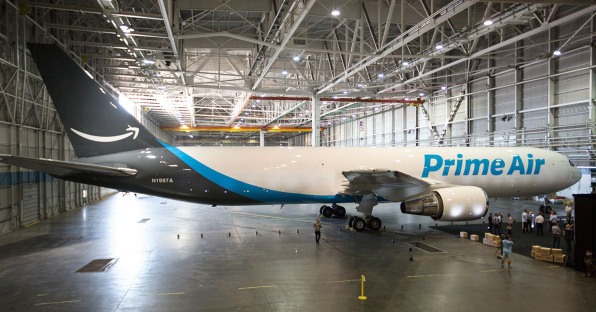
\includegraphics[width=.6\paperwidth]{prime-air.jpg}
{\scriptsize \caption{Immagine utilizzata come riferimento in questo confronto.}
\label{fig:riconscimento-oggetti-ambientazione}}
\end{center}
\end{figure}
%

Da aggiungere che le Microsoft Computer Vision generano anche la seguente descrizione: ``A large airplane at an airport''.

Come si può vedere dalla tabella, tutte le API identificano relativamente bene gli elementi principali dell'immagine
(l'hangar, l'aereo), eccetto per le Visual Recognition (IBM) che non riconosce l'aereo.
%
\begin{table}[!h]
\centering
{\footnotesize
\resizebox{.8\textwidth}{!}{
\begin{tabularx}{.8\textwidth}{l|l|l|l}
\toprule
Computer Vision   			& Visual Recognition     		& Reckognition 					& Cloud Vision 				\\ \hline
\midrule
plane (97,41\%)            & hangar (97,9\%)           	  & Hangar (95,74\%)               & Airliner (96\%)             \\
indoor (96,20\%)               & blue color (85,9\%)       & Aircraft (89,96\%)             & Airline (95\%)              \\
floor (96,10\%)                & steel blue color (75,5\%) & Airplane (89,96\%)             & Airplane (95\%)             \\
airplane (91,19\%)             &                           & Warplane (66,30\%)             & Vehicle (91\%)              \\
airport (91,11\%)              &                           & Jet (57,09\%)                  & Air travel (90\%)           \\
aircraft (72,66\%)             &                           & Landing (52,80\%)              & Aircraft (87\%)             \\
transport (67,56\%)            &                           &                                & Aviation 85\%)              \\
\bottomrule
\end{tabularx}}
\caption{Tabella riassuntiva per il riconscimento oggetti e ambientazione.}
\label{tab:riconscimento-oggetti-ambientazione}}
\end{table}
%
\paragraph{Classificazione}\label{par:esempi-classificazione}
Si consideri sempre una'immagine raffigurante un oggetto predominante nell'immagine con l'obbiettivo di classificarlo.
Prendiamo l'immagine di esempio in Figura~\ref{fig:riconscimento-classificazione} e utilizziamo le Computer Vision API
di Microsoft e le Visual Recognition di IBM (le piattaforme Google e Amazon non forniscono un sistema di classificazione in categorie).

\noindent
\begin{minipage}[b]{0.38\textwidth}
	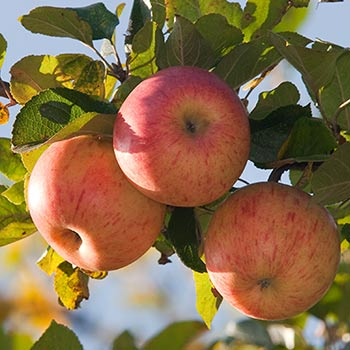
\includegraphics[width=.8\linewidth]{esempi-vari/mele.jpg}
	\label{fig:riconscimento-classificazione}
\end{minipage}
\hfill
\begin{minipage}[b]{0.6\textwidth}
	Computer Vision: \textsf{Object} $\rightarrow$ \textsf{Plant} $\rightarrow$ \textsf{Flower};\\
	Visual Recognition:
	\begin{itemize}
		\item \textsf{fruit} $\rightarrow$ \textsf{pome} $\rightarrow$ \textsf{eating apple} $\rightarrow$ \textsf{Macoun}\footnote{Le
		mele Macoun sono una varietà di mele commestibili: \href{https://en.wikipedia.org/wiki/Macoun_apple}{Mele Macoun}.};
		\item \textsf{plant} $\rightarrow$ \textsf{apple tree}.
	\end{itemize}
	\vfill
\end{minipage}
\noindent
%
\paragraph{Riconoscimento di testo}\label{par:riconscimento-testo}
In questo esempio verrà presentato il riconoscimento di testo scritto a mano libera (più difficile rispetto al testo scritto a macchina).

\begin{minipage}[b]{0.38\textwidth}
	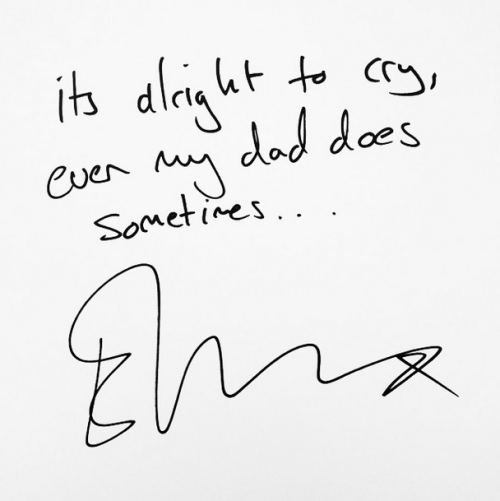
\includegraphics[width=.8\linewidth]{esempi-vari/testo.png}
	\label{fig:riconscimento-testo}
\end{minipage}
\hfill
\begin{minipage}[b]{0.6\textwidth}
	\begin{itemize}
		\item Computer Vision:
			{\footnotesize
			\begin{quote}
				It's alright to cry\\
				even my dad does\\
				Sometimes
			\end{quote}}
			\item Visual Recognition e Reckognition: funzionalità non presente;
			\item Cloud Vision:
			{\footnotesize
			\begin{quote}
				is dle at to CCS, even a dod does MA Sometimes
			\end{quote}}
		\end{itemize}
	\vfill
\end{minipage}
\noindent
Come si può vedere le Computer Vision sono le uniche a riconscere la quasi totalità del testo (mancano solo i segni di punteggiatura), mentre le Cloud Vision
rilevano il testo ma grossi con errori (tali da compromettere il significato finale).
Amazon e IBM, invece, rilevano la presenza di testo ma non riconoscono le parole/lettere (infatti non hanno la funzionalità di riconscimento del testo).
%
\paragraph{Riconoscimento di contenuti non adatti ai minori}\label{par:riconscimento-racy}
Con questo esempio si vuole vedere come, e in che grado, un'immagine viene classificata come ``non adatta ai minori''\footnote{Contenuto pornografico e/o erotico.}.
Con questo obbiettivo in mente, sono state identificate le due immagini in Figura~\ref{fig:riconscimento-racy}: entrambe le due immagini potrebbero essere identificate
come a contenuto erotico (difficilmente come pornografico).
\begin{figure}[!h]
\begin{center}
	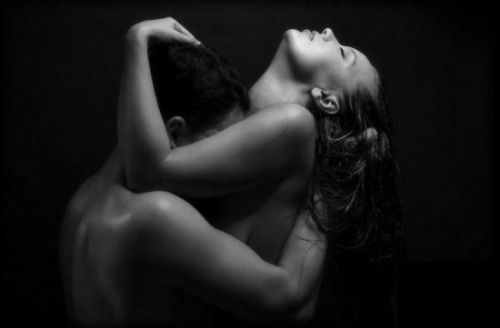
\includegraphics[width=.39\linewidth]{esempi-vari/racy-1.jpg}
	\hfill
	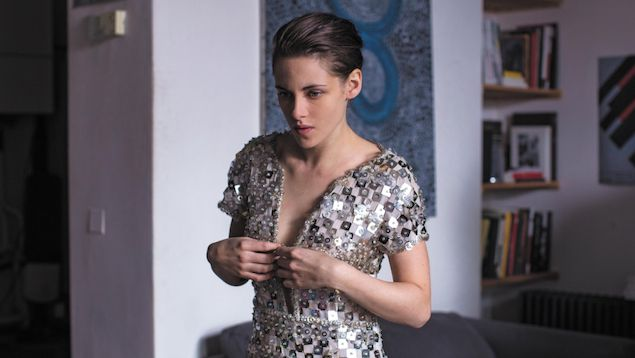
\includegraphics[width=.59\linewidth]{esempi-vari/racy-2.jpg}
{\scriptsize \caption{Immagini utilizzate come riferimento.}
\label{fig:riconscimento-racy}}
\end{center}
\end{figure}
%
Dai risultati si osserva che:
\begin{itemize}
	\item Computer Vision: identifica solo la prima immagine (quella di sinistra) come erotica;
		Per questa si hanno entrambi i campi \textsf{isAdultContent} e \textsf{isRacyContent} veri e
		\textsf{racyScore} al 73,88\%; per l'immagine di destra, invece, i primi campi sono falsi
		e il terzo è pari a 7,28\%.
	\item Visual Recognition: funzionalità non presente;
	\item Reckognition: la prima immagine viene etichettata come ``contenuto per adulti'' e ``svestiti'' (\textit{Suggestive} e \textit{Revealing Clothes}) con un
	livello di confidenza del 53,30\%, mentre nella seconda non viene rilevato niente (nessun contenuto per adulti).
	per la prima immagine sono stati trovate le etichette
	\item Cloud Vision: contenuto come ``per adulti'' (\textit{Adult}) con valore \textsf{Possible} (ricordarsi la scala valori delle Cloud Vision) per la prima immagine;
	niente per la seconda.
\end{itemize}
Dai risultati sopra ottenuti si vede come tutti i servizi che presentato questa funzionalità hanno identificato (con un grado più o meno elevato)
la prima immagine come contenente contenuti per adulti, mentre non ne sono stati trovati per la seconda.
%
\paragraph{Riconoscimento di personaggi famosi}\label{par:riconscimento-celebrita}
Una funzionalità comune a tutte la piattaforme è il riconscimento di celebrità e/o personaggi famosi.
Come si nota dai risultati in Tabella~\ref{tab:riconscimento-celebrita}, la persona raffigurata in Figura~\ref{fig:riconscimento-celebrita}
è stata quasi sempre identificata con il grado di affidabilità massimo (o quasi).
Da notare che Visual Recognition non ha riconosciuto il personaggio\footnote{A essere precisi, il personaggio scelto non è una celebrità
ma un personaggio pubblico (anche se molto conosciuto).}.
\begin{figure}[!h]
\begin{center}
	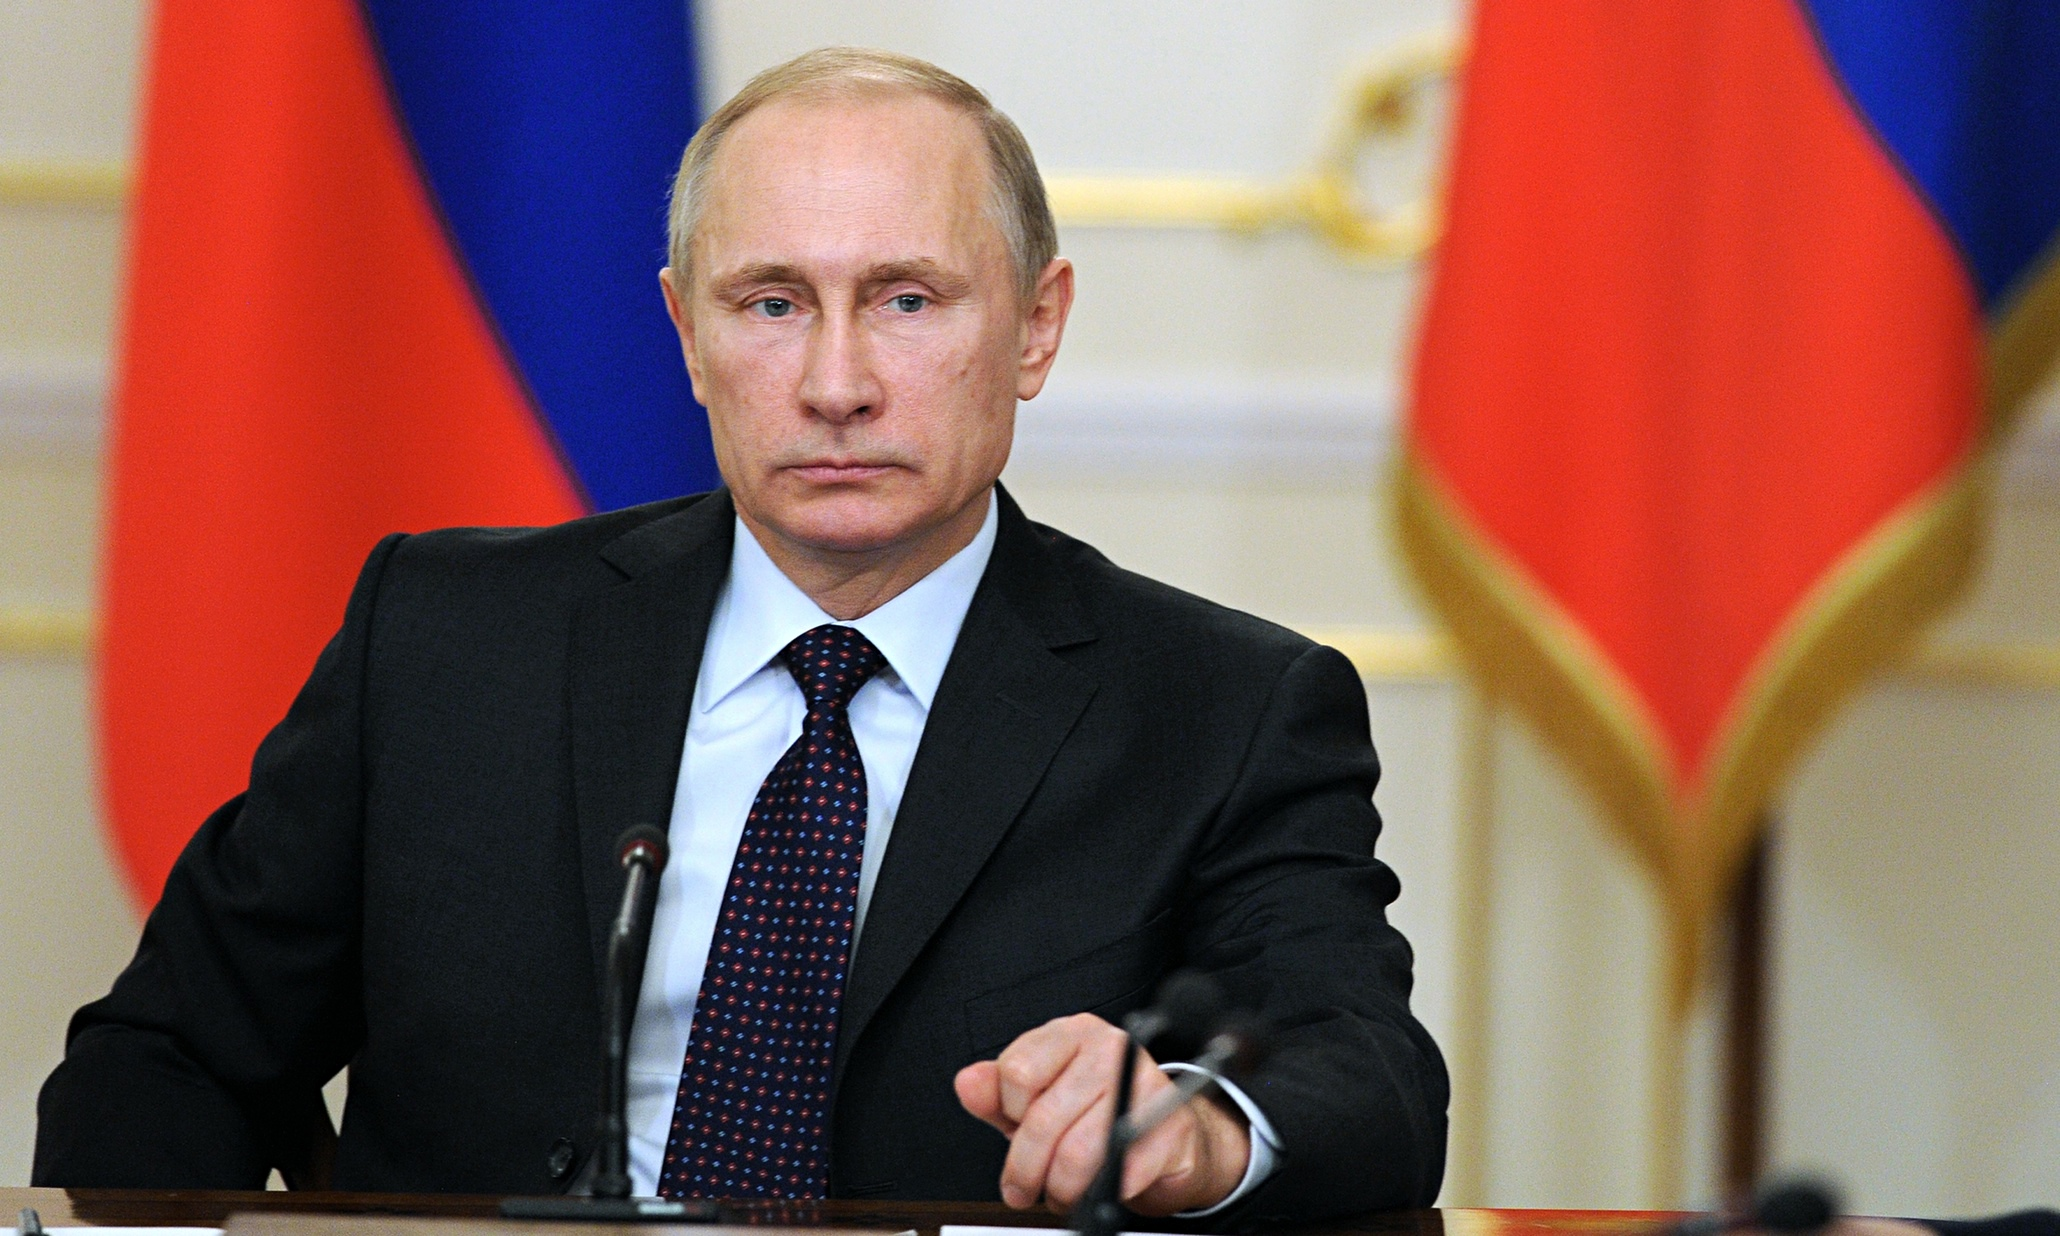
\includegraphics[width=.7\textwidth]{esempi-vari/putin.jpg}
{\scriptsize \caption{Immagine utilizzata come riferimento.}
\label{fig:riconscimento-celebrita}}
\end{center}
\end{figure}
%
\begin{table}[!h]
\centering
{\footnotesize
\resizebox{.8\textwidth}{!}{
\begin{tabularx}{.8\textwidth}{c?l|l|l|l}
\toprule
						& Computer Vision   			& Visual Recognition     		& Reckognition 					& Cloud Vision 				\\ \hline
\midrule
Nome					& Vladimir Putin				& Maschio generico				& Vladimir Putin				& Vladimir Putin			\\
Affidabilità			& 100\%							& 97\%							& 99\%							& -							\\
\bottomrule
\end{tabularx}}
\caption{Tabella riassuntiva per il riconscimento di personaggi famosi.}
\label{tab:riconscimento-celebrita}}
\end{table}
%
\paragraph{Riconoscimento luoghi di interesse}\label{par:riconscimento-luoghi-interesse}
Anche in questo caso sono state identificate due immagini, una raffigurante un luogo storico naturale e l'altra
un monumento artificiale.
Come si può vedere in Figura~\ref{fig:riconscimento-luoghi-interesse}, sono state scelte le immagini raffiguranti
le Cascate del Niagara\footnote{\href{https://it.wikipedia.org/wiki/Cascate_del_Niagara}{Wikipedia: Cascate del Niagara}.} e
la Piramide di Chefren\footnote{\href{https://it.wikipedia.org/wiki/Piramide_di_Chefren}{Wikipedia: Piramide di Chefren}.},
due luoghi molto famosi e conosciuti.
%
\begin{figure}[!h]
\begin{center}
	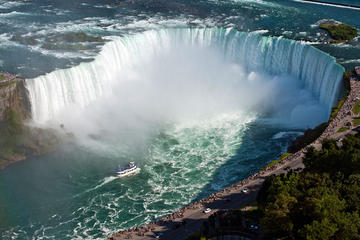
\includegraphics[width=.49\linewidth]{esempi-vari/landmark-1.jpg}
	\hfill
	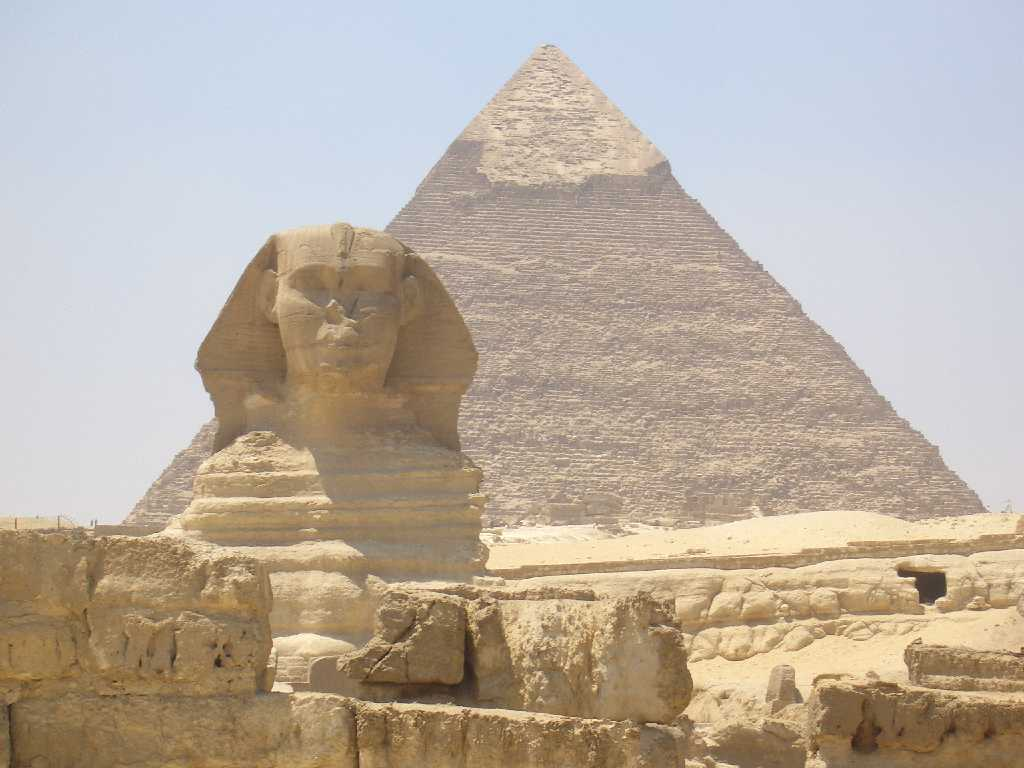
\includegraphics[width=.49\linewidth]{esempi-vari/landmark-2.jpg}
{\scriptsize \caption{Immagini utilizzate come riferimento.}
\label{fig:riconscimento-luoghi-interesse}}
\end{center}
\end{figure}
L'unica piattaforma a riconoscere entrambe le immagini è stata Google (Cloud Vision) identificandole correttamente.
Le Vision Recognition (IBM) hanno identificato correttamente solo la seconda immagine.
Per quanto riguarda gli altri servizi, invece, hanno riconosciuto gli elementi presenti in generale (cascate, ambiente aperto, montagna o piramidi per la seconda)
ma non il luogo in particolare.
%
\paragraph{Riconoscimento di un volto}\label{par:riconscimento-singolo-volto}
In questo confronto lo scopo era quello di verificare le caratteristiche del volto (\textit{landmark}) che l'API era in grado di riconsoscere in un ambiente semplice;
per questo motivo è stata scelta un'immagine di un primo piano di una ragazza\footnote{I diritti dell'immagine sono del legittimi proprietario.}.
Come si può notare dai risultati in Figura~\ref{fig:riconscimento-singolo-volto}, tutte le API hanno riconosciuto e identificato correttamente il volto e, a parte
il servizio offerto da IBM, diversi elementi di questo.
Il migliore di questi sembrerebbe essere le API di Google che, tuttavia, non fornisce indicazioni sulla persona specifica (età, sesso).
\begin{figure}[!h]
\begin{center}
	\includegraphics[width=.2\linewidth]{riconoscimento-viso-1/microsoft.jpg}
	\includegraphics[width=.2\linewidth]{riconoscimento-viso-1/ibm.jpg}
	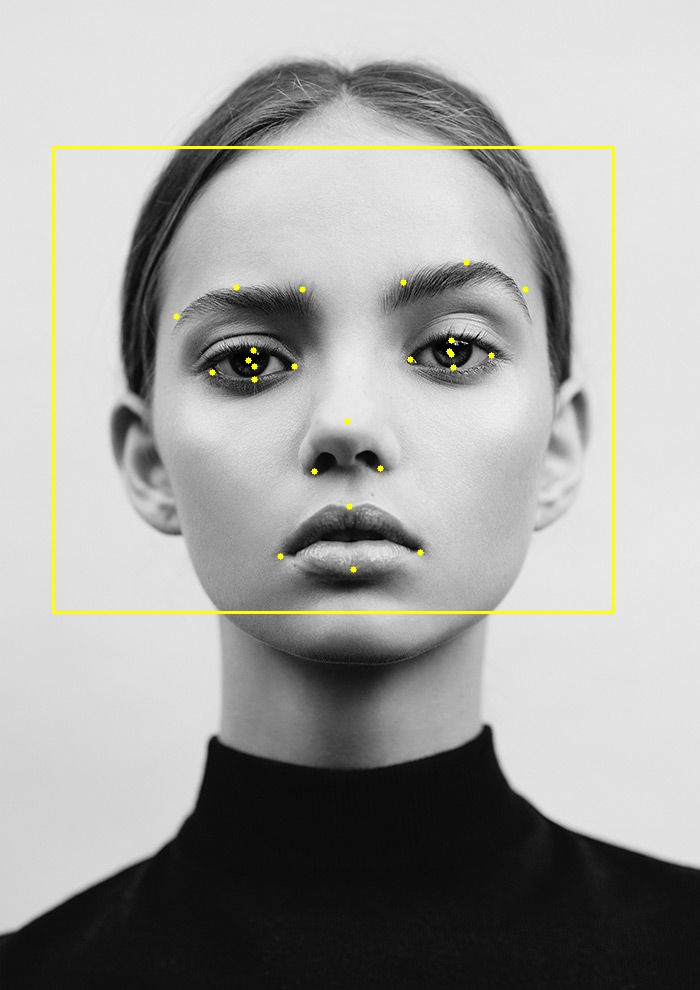
\includegraphics[width=.2\linewidth]{riconoscimento-viso-1/amazon.jpg}
	\includegraphics[width=.2\linewidth]{riconoscimento-viso-1/google.png}
{\scriptsize \caption{Riconscimento di un singolo volto utilizzando le API di (da sinistra): Microsoft, IBM, Amazon, Google. (Fonte: \url{http://eddienew.com})}
\label{fig:riconscimento-singolo-volto}}
\end{center}
\end{figure}
%
\paragraph{Riconoscimento di più volti}\label{par:riconscimento-volti-multipli}
Come si vede dalla Figura~\ref{fig:riconscimento-volti-multipli}, quasi tutti i volti nella foto sono stati riconosciuti.
Da notare come le API Amazon riescano anche a determinare l'orientamento dei singoli volti.
\begin{figure}[!h]
\begin{center}
	\includegraphics[width=.4\linewidth]{riconoscimento-viso-2/microsoft.jpg}
	\includegraphics[width=.4\linewidth]{riconoscimento-viso-2/ibm.jpg}
	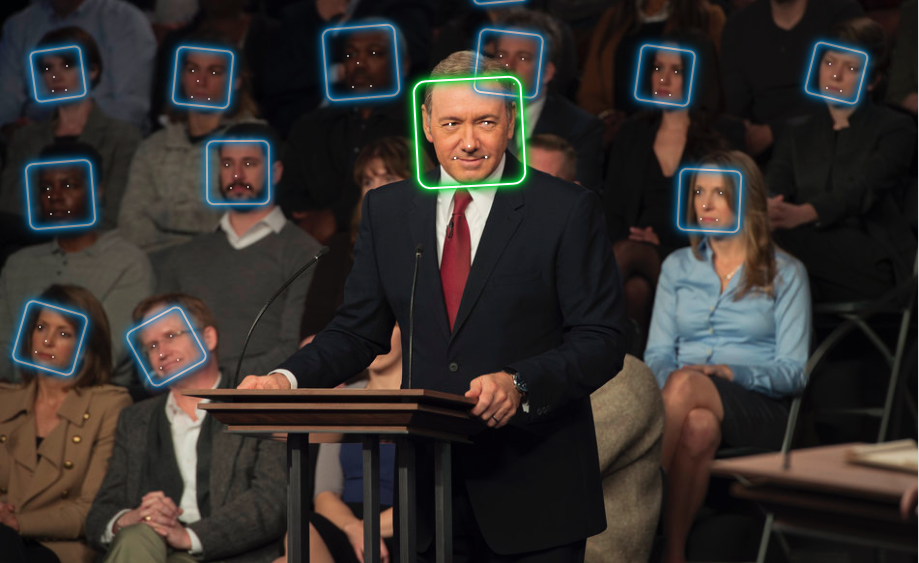
\includegraphics[width=.4\linewidth]{riconoscimento-viso-2/amazon.png}
	\includegraphics[width=.4\linewidth]{riconoscimento-viso-2/google.png}
{\scriptsize \caption{Riconscimento di più singolo volto utilizzando le API di (da sinistra): Microsoft, IBM, Amazon, Google.}
\label{fig:riconscimento-volti-multipli}}
\end{center}
\end{figure}
%
